% !TeX root = ./AER Insights.tex
% Last updated:
% 5 Aug 18 - CC
%%%%%%%%%%% APPENDIX EXHIBITS

% A. Empirical Setting Details \label{app:emp_setting} 
% Table A.1 Summary stats for RAIS sample \label{tab:rais_sum}
% Table A.2 Summary stats for RAIS-WMS match \label{tab:wms_summ}
\section{Data Sources}
\label{app:EmpiricalDetails}

\subsection{The \emph{Rela\c{c}\~{a}o Anual de Informa\c{c}\~{o}es Sociais} (RAIS)}
We use matched employer-employee data from Brazil's \emph{Rela\c{c}\~{a}o Anual de Informa\c{c}\~{o}es Sociais} (RAIS) for the period 2003-2013.
The RAIS is an administrative census of all jobs in Brazil covered by a formal contract. Each year, the Brazilian Ministry of Labor and Employment (MTE) collects data from each establishment on every employment contract that was active during the calendar year. For businesses, reporting the data under RAIS is mandated by the constitution. Hence, compliance with reporting requirements is extremely high, as employers who fail to complete the survey face mandatory fines and also risk litigation from employees, to whom the company must make mandatory leave-loading and social security payments.

For each job, in each year, the employer reports characteristics of the worker, the job, and the establishment. 
Worker characteristics include gender, race, age, and educational attainment.\footnote{ 
Because individual characteristics are reported by the employer, they can change as workers move from job to job. 
\citet*{CRS:Race:JHR:2017} provide evidence that discrepancies in employers' reports of worker characteristics are associated with other unobserved determinants of earnings, so we leave these variables in as reported.} 
Job characteristics relevant to this study include the monthly wage, weekly contracted hours, occupation, and the cause of job separations (which we use to distinguish voluntary and involuntary separations.) Establishment characteristics include the establishment's industry, location, and number of employees. 

\subsection{Distinguishing Managers and Production Workers in RAIS}
% [TO FINISH]
In RAIS, We are able to distinguish workers holding managerial positions from production workers.
Each contract-year observation includes a variable that reports the 5-digit occupation code according to the Brazilian classification system, the \emph{Classificaç{\~a}o Brasileira de Ocupaç{\~o}es} (CBO).\footnote{Detailed information on the CBO classification system is available via \href{http://www.mtecbo.gov.br}{http://www.mtecbo.gov.br}.} 
Under the CBO, occupations with the first digit `1' correspond to  ``Membros superiores do poder p\'{u}blico, dirigentes de organiza\c{c}\~{o}es
 de interesse p\'{u}blico e de empresas e gerentes'' (Leaders of public agencies, and directors and managers of organizations and businesses). We therefore classify as managerial all jobs with first digit of CBO code equal to 1.

 We find that many of the establishments in RAIS do not have any workers in occupations classified as managerial according to the rule above. Hence, we expand our classification of managers in two ways.  We use the third digit of the occupation code, which indicates hierarchical level. Specifically, a third digit of `0` in the CBO code indicates the position is supervisory over the jobs in the corresponding two-digit group. For example, occupations classified with leading digits ``52'' are ``vendors of commerical services.'' Occupations with leading digits ``520'' are ``supervisors of vendors of commercial services.'' We classify all such supervisory occupations as managerial. %Second, in the WMS data, we know the survey respondent is a manager or director. While the WMS does not record the CBO occupation of the respondent, ... [TO FINISH]
  
   
 


\subsection{Formal Employment in Brazil}
In Brazil a worker is formally employed if he or she has a registered identification number with one of two social security programs: the \emph{Programa de Integra\c{c}\~{a}o Social} (PIS), or Social Integration Program, or the \emph{Programa de Forma\c{c}\~{a}o do Patrim\^{o}nio do Servidor P\'{u}blico} (PASEP), or Civil Servants Equity Formation Program, depending on whether the worker is employed in the private sector or the public sector. PIS/PASEP numbers are consistent across workers and follow a worker for life. For firms, formal employment means that the employer contributes the \textit{Abono Salarial} along with other social security payments to a bank account administered by either \emph{Caixa Econ\^{o}mica Federal} if registered with PIS, or \emph{Banco do Brasil} for PASEP workers. Formal employers must also have employment contracts for all employees. The most common contract type is the \emph{Consolida\c{c}\~{a}o das Leis de Trabalho} (CLT), or Labor Law Consolidation. Other formal employment relationships include internships, independent contracting, directorships and government contracts, but we do not consider these types of contract in this paper.
% The Brazilian government defines formal employment with these criteria, and this definition is consistent with definitions used by researchers when studying other Latin American economies \citep{Gasparini2009}. 
The number of formal contracts grew steadily in Brazil during our sample period, from nearly 42 million jobs in 2003 to over 72 million jobs in 2010. Unemployment decreased from eleven percent to five percent, and real wages grew over the period as well. Our sample therefore covers a period of growth and tightening labor-market conditions.

\subsection{Preparation of the RAIS Analysis Data}
\label{sec:RAIS_analysis_description}
We base our analysis on an extract of the full RAIS data with several restrictions.
For workers with multiple jobs in a given year, we focus on the job with the highest total earnings in that year, based on the reported number of months worked and the average monthly earnings.
We also restrict attention to jobs with at least 30 hours contracted hours per week.
Using this unbalanced panel of workers, we drop all observations in plants with fewer than five workers, and observations with missing data on tenure or earnings. 
Finally, we drop all observations where the job is reported to be some form of government contract.

Table \ref{tab:rais_sum} provides basic descriptive statistics summarizing our main analysis file assembled from the raw RAIS data.

\section{Additional Details of the Firm-level Data}

We show the distribution of the skill of managers and of production workers, as measured by the AKM worker effect, in Figure \ref{fig:pe_kdensity}.
Managers clearly have much higher average skill, but also higher variance. The distribution of managerial skill is also highly skewed. The skill distribution for production workers is approximately log-normal. The distribution of manager skill has a very fat right-tail, indicating the presence of many highly-paid managers. Moreover, the distribution shows some evidence of being bi-modal.

%\section{Details of Production Function Estimation}
%[IN PROGRESS]
% C. Production Function Estimation \label{app:prod_fn}
% Table C.1 Summary stats for production data \label{tab:prod_stats}
% Table C.2 Production function estimates \label{tab:prod_est}

\clearpage
\section{Appendix Tables and Figures}
% IM Schmutte
% RAIS_sum.tex
% Summary table of estimated components from AKM estimation
%SOURCE: E:\Dropbox\MGMT_source\data\_dev\programs\prepare\04.03.RAIS_descriptive_statistics.sas (lst)

\begin{table}[h t]										
    \begin{center}									
    \caption{Summary of RAIS 2003--2013 \label{tab:rais_sum}}										
        \begin{tabular}{l r r}										
            \toprule
                Variable & Mean Std.\ & Dev. \\
            \midrule
                Log Wage	        & $1.65$	& $0.69$  \\
                Log Monthly Earn.	& $6.87$	& $0.67$  \\
                White	            & $0.59$	& $0.49$  \\
                Male                & $0.64$	& $0.48$  \\
                Age	                & $33.24$	& $10.59$  \\
                age $\le$ 30	        & $0.48$	& $0.50$  \\
                age $\ge$ 50	        & $0.09$	& $0.28$  \\
                Work Hours          & $43.12$	& $2.58$  \\
                Hours $\ge$ 35        & $0.98$	& $0.13$  \\
            \bottomrule
        \end{tabular}
    \end{center}
    \footnotesize{Notes: Summary statistics of the RAIS data used to estimate the AKM decomposition. 
    The data are a worker-year panel constructed from the raw RAIS job-year files. We assign workers to the job with highest reported earnings over the year.
    We also drop all worker-year observations where the number of reported jobs is greater than 2.
    We drop jobs with fewer than 30 contracted hours per week, jobs in the public sector, jobs in plants with fewer than 5 workers, and jobs with missing data
    on tenure or earnings. The final number of observations is $N = 353,141,951$.}
\end{table}										
							

\clearpage
\begin{table}[h t]
    \caption{ \label{tab:wms_summ}}
    \begin{center}
    \scalebox{0.7}{
        {
\def\sym#1{\ifmmode^{#1}\else\(^{#1}\)\fi}
\begin{tabular}{l*{1}{cccccc}}
\toprule
                    &\multicolumn{6}{c}{}                                                         \\
                    &\textbf{Mean}&\textbf{Median}&\textbf{Min}&\textbf{Max}& \textbf{SD}&  \textbf{N}\\
\midrule
\textbf{Firm characteristics}&            &            &            &            &            &            \\
Number of employees (WMS)&      600.78&       300.0&        40.0&      5000.0&    (816.49)&         961\\
Number of production sites, total (WMS)&        3.79&         1.0&         0.0&        91.0&      (9.40)&         961\\
Number of production sites, abroad (WMS)&        2.28&         0.0&         0.0&       100.0&     (11.05)&         961\\
Firm age (WMS)      &       36.42&        33.0&         1.0&       316.0&     (25.55)&         961\\
Firm has no competitors (WMS)&        0.01&         0.0&         0.0&         1.0&      (0.08)&         961\\
Firm has less than 5 competitors (WMS)&        0.23&         0.0&         0.0&         1.0&      (0.42)&         961\\
Firm has 5 or more competitors (WMS)&        0.76&         1.0&         0.0&         1.0&      (0.43)&         961\\
Firm is family owned (WMS)&        0.26&         0.0&         0.0&         1.0&      (0.44)&         961\\
Firm is founder owned (WMS)&        0.36&         0.0&         0.0&         1.0&      (0.48)&         961\\
Firm is institutionally owned (WMS)&        0.05&         0.0&         0.0&         1.0&      (0.22)&         961\\
Firm is non-family privately owned (WMS)&        0.16&         0.0&         0.0&         1.0&      (0.36)&         961\\
Firm is owned by dispersed shareholders (WMS)&        0.14&         0.0&         0.0&         1.0&      (0.34)&         961\\
Other ownership (WMS)&        0.04&         0.0&         0.0&         1.0&      (0.19)&         961\\
Firm is a multinational (WMS)&        0.21&         0.0&         0.0&         1.0&      (0.41)&         961\\
Firm is a domestic multinational (WMS)&        0.01&         0.0&         0.0&         1.0&      (0.11)&         961\\
Hierarchy: layers between CEO and shopfloor (WMS)&        3.33&         3.0&         1.0&         8.0&      (1.15)&         961\\
Span of control: number of direct reports (WMS)&        7.09&         6.0&         1.0&        30.0&      (5.01)&         961\\
\textbf{Management scores}&            &            &            &            &            &            \\
Overall management score, raw (WMS)&        2.70&         2.7&         1.1&         4.7&      (0.65)&         961\\
Operations management score, raw (WMS)&        2.44&         2.5&         1.0&         5.0&      (1.02)&         961\\
Monitoring management score, raw (WMS)&        3.08&         3.2&         1.0&         5.0&      (0.81)&         961\\
Target management score, raw (WMS)&        2.63&         2.6&         1.0&         5.0&      (0.78)&         961\\
People management score, raw (WMS)&        2.52&         2.5&         1.0&         4.7&      (0.58)&         961\\
\textbf{Worker characteristics}&            &            &            &            &            &            \\
Share of female managers (WMS)&        0.18&         0.1&         0.0&         1.0&      (0.19)&         480\\
Share of female non-managers (WMS)&        0.30&         0.3&         0.0&         1.0&      (0.24)&         480\\
Share of female workers, total (WMS)&        0.30&         0.3&         0.0&         1.0&      (0.24)&         480\\
Share of female workers, total (RAIS)&        0.29&         0.2&         0.0&         1.0&      (0.22)&         961\\
Age of workers (RAIS)&       33.05&        32.7&        21.0&        53.0&      (3.75)&         961\\
Weekly hours worked (RAIS)&       43.51&        44.0&        30.0&        44.0&      (1.29)&         961\\
Weekly hours worked (WMS)&       43.80&        44.0&        35.0&        65.0&      (2.47)&         961\\
Weekly hours worked, managers (WMS)&       48.68&        45.0&        35.0&        80.0&      (7.06)&         961\\
Weekly hours worked, non-managers (WMS)&       43.63&        44.0&        35.0&        65.0&      (2.45)&         961\\
Employee tenure, weeks (RAIS)&       43.98&        39.8&         2.9&       213.7&     (22.12)&         961\\
Hourly wage, BRL Reais (RAIS)&       11.24&         8.3&         2.5&       159.7&     (10.61)&         961\\
Monthly earnings, BRL Reais (RAIS)&     2079.36&      1530.3&       463.4&     30120.6&   (1931.22)&         961\\
\textbf{Worker education}&            &            &            &            &            &            \\
Share of managers with university degree (WMS)&        0.73&         0.9&         0.0&         1.0&      (0.33)&         961\\
Share of non-managers with university degree (WMS)&        0.10&         0.1&         0.0&         1.0&      (0.13)&         961\\
Share of employees with university degree (WMS)&        0.13&         0.1&         0.0&         1.0&      (0.13)&         961\\
Share of employees with university degree (RAIS)&        0.13&         0.1&         0.0&         1.0&      (0.18)&         961\\
Share of employees with high school degree (RAIS)&        0.55&         0.6&         0.0&         1.0&      (0.21)&         961\\
\bottomrule
\end{tabular}
}

    }
    \end{center}
    \footnotesize{Notes: Summaries of the matched WMS-RAIS panel. The dataset is a firm-year panel with one observation for each WMS firm in each year it was surveyed
    and can be matched to RAIS. There are 694 unique firms. Of these, 267 were surveyed in both years, 213 were surveyed only in 2008, and 214 were surveyed only in 2013. 
    The data also include firm-level summaries of RAIS variables. Note that the WMS only asked Brazilian firms about gender composition in 2013, which explains the discrepancies in the
    number of observations for those variables.}
\end{table}

\clearpage
% Ian M. Schmutte
% dynamic_selection.tex
% This version: 29 Oct 2018
% Changes over time in the sample of WMS/RAIS matched firms from 2003--2008
%SOURCE: Dropbox\MGMT_source\data\_dev\programs\analysis\emp_shares.log


\begin{table}[h t]
	\caption{Composition of Establishments in RAIS-WMS Data: 2003--2013 \label{tab:dynamic_selection}}
	\begin{center}
	\begin{tabular}{l ccc}																					
        \toprule		
                            &     (1)           &    (2)                &    (3)          \\
                             & 	\m{Share}	&	\m{Management}	&	\m{Plant}  \\
                    Year    &   \m{Active}       &   \m{Score}          &   \m{Effect} \\
        \midrule    
		            2003    &  $0.88$           &    $-.011$                   & $.155$            \\
                    2004    &  $0.91$           &    $-.025$                   & $.151$      \\
                    2005    &  $0.94$           &    $-.033$                   & $.157$      \\
                    2006    &  $0.95$           &    $-.017$                   & $.160$      \\
                    2007    &  $0.95$           &    $-.010$                   & $.160$      \\
                    2008    &  $0.95$           &    $-.011$                   & $.150$      \\
                    2009    &  $0.93$           &    $-.006$                   & $.151$      \\
                    2010    &  $0.92$           &    $-.003$                   & $.152$      \\
                    2011    &  $0.94$           &    $0.004$                   & $.154$      \\
                    2012    &  $0.93$           &    $0.022$                   & $.167$      \\
                    2013    &  $0.91$           &    $0.027$                   & $.169$      \\
		\bottomrule 
	\end{tabular}
	\end{center}
	\footnotesize{Notes: Table entries are summaries of characteristics of 728 establishments from WMS that can be matched to at least one year of RAIS between 2003--2013. Column (1) reports the share of these 728 establishments observed in a given year. Columns (2) reports the average standardized management score, which is centered on zero with standard deviation 1. Column (3) reports the average estmated establishment effect across firms observed in a given year. }

\end{table}



























\clearpage
\begin{figure}
    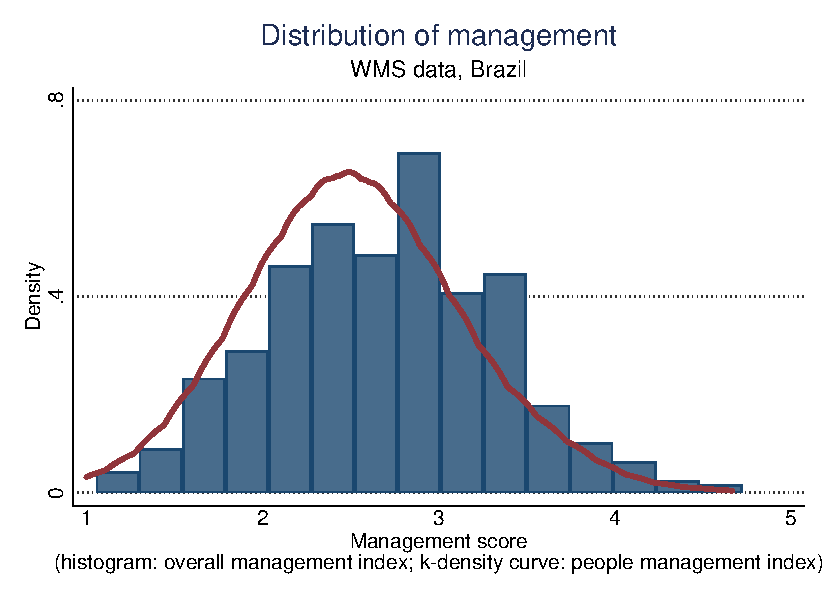
\includegraphics[width = 0.9\textwidth]{../../../figures/mgmtscor_hist}
    \caption{Distribution of overall management score (histogram) and people management score (kernel density) for Brazilian plants surveyed in 2008 or 2013.}
    \label{fig:pe_kdensity}
\end{figure}

\clearpage
%tab_prodfcn_2008_old.tex
%Ian M. Schmutte
% 2018-10-29
% Uses results from C:\Users\schmutte\Dropbox\MGMT_source\output\IBGE\igbe_summary.tex
\begin{table}
\caption{Descriptive Statistics: WMS-RAIS-PIA Matched Data} \label{tab:WMSRAISPIA_sumstats}
\scalebox{0.8}{
\begin{tabular}{lllllll}
\toprule
 & Mean & 25th p & Median & 75th p & Std.\ Dev. & Num.\ Obs. \\
\midrule
Multinational status & 0.21 & 0 & 0 & 0 & 0.41 & 685 \\
Avg share of union members & 51.34 & 10 & 50 & 95 & 39.02 & 684 \\
Firm age & 35.5 & 18 & 31 & 46 & 25.61 & 685 \\
Avg number of reported competitors & 7.37 & 4 & 10 & 10 & 3.11 & 685 \\
Share of female workers & 30.64 & 13.34 & 28.2 & 45.6 & 22 & 675 \\
Share of family firms (Orbis) & 0.44 & 0 & 0 & 1 & 0.5 & 19595 \\
Share of private firma (WMS) & 0.19 & 0 & 0 & 0 & 0.39 & 685 \\
Share of institutional firms (WMS) & 0.07 & 0 & 0 & 0 & 0.26 & 685 \\
Share of founder firms (WMS) & 0.36 & 0 & 0 & 1 & 0.48 & 685 \\
Share of family firms (WMS) & 0.25 & 0 & 0 & 1 & 0.43 & 685 \\
Share workers with college degree & 0.07 & 0 & 0.02 & 0.07 & 0.13 & 19788 \\
Avg share of high school educated workers & 0.41 & 0.2 & 0.39 & 0.58 & 0.26 & 19788 \\
Avg share of white workers & 0.71 & 0.56 & 0.82 & 0.95 & 0.3 & 19788 \\
Log of wage mean (RAIS) & 1.74 & 1.39 & 1.69 & 2.01 & 0.5 & 19788 \\
Separation mean (RAIS) & 0.28 & 0.18 & 0.26 & 0.36 & 0.16 & 19788 \\
\# employees & 260.49 & 60 & 91 & 180 & 1065.05 & 20056 \\
Log employees & 4.76 & 4.14 & 4.54 & 5.23 & 1.05 & 19263 \\
% Capital & 72056829.28 & 295724.81 & 3325481 & 16378560 & 1.96E+09 & 19537 \\
Log capital & 13.4 & 12.6 & 15.02 & 16.61 & 5.47 & 19537 \\
% Materials & 62882504.6 & 1227372.13 & 6746602.5 & 23828716 & 7.82E+08 & 19335 \\
Log materials & 15.49 & 14.04 & 15.73 & 16.99 & 2.32 & 19272 \\
\bottomrule
\end{tabular}
}

\footnotesize{Notes: Summaries of variables in the WMS-RAIS-PIA matched data. The variables are from PIA, except where noted. Variables from WMS are only available for WMS firms, as reflected in the number of observations.
\end{table}

\clearpage
\begin{figure}
    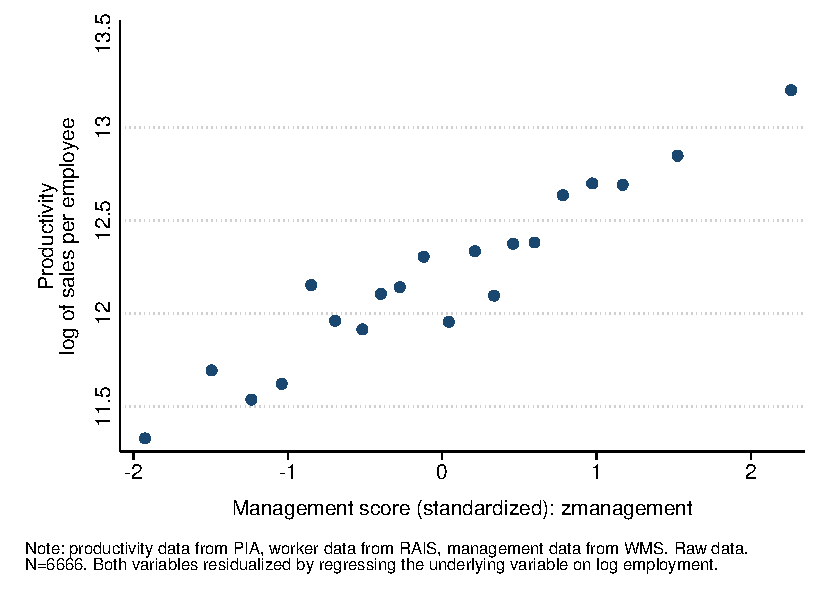
\includegraphics[width=0.9\textwidth]{../../../IBGE/figs/cvb_fig5_zmanagement}
    \caption{Relationship between sales and WMS management score}
    \label{fig:sales_v_mgmt}
\end{figure}

\clearpage
\begin{figure}
    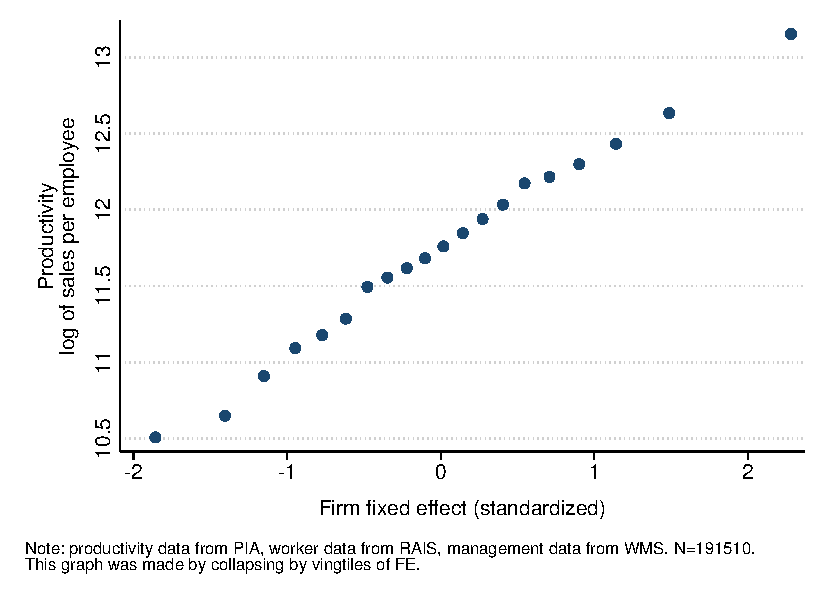
\includegraphics[width=0.9\textwidth]{../../../IBGE/figs/cvb_fig7a_sa}
    \caption{Relationship between sales and estimated AKM firm effect}
    \label{fig:sales_v_fe}
\end{figure}

\clearpage
\begin{figure}
    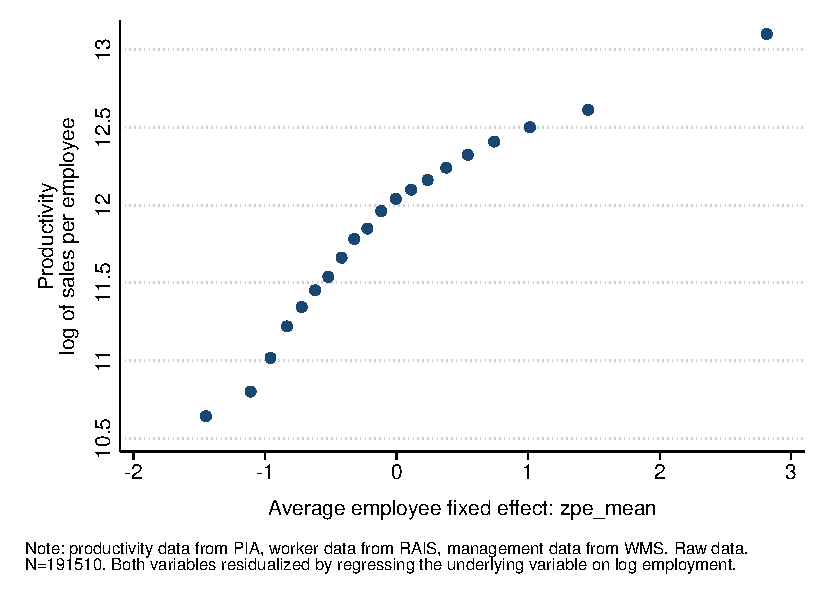
\includegraphics[width=0.9\textwidth]{../../../IBGE/figs/cvb_f6_zpe_mean_sa}
    \caption{Relationship between sales and average estimated AKM worker effect}
    \label{fig:sales_v_pe}
\end{figure}

\clearpage
\begin{figure}
    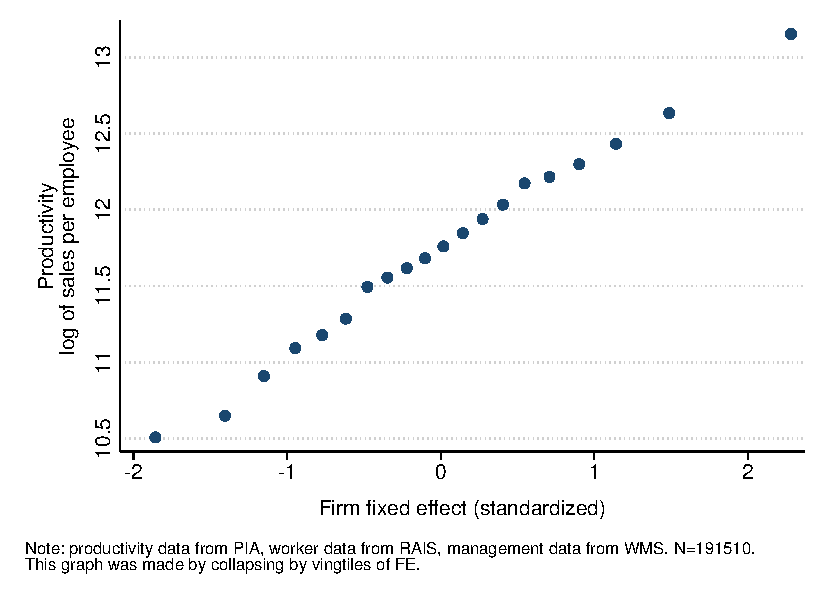
\includegraphics[width=0.9\textwidth]{../../../IBGE/figs/cvb_fig7a_sa}
    \caption{Relationship between sales and estimated AKM firm effect}
    \label{fig:sales_v_fe}
\end{figure}


\clearpage
%Ian M. Schmutte
% 2018 Aug 4
%source /projects/schmutte/MGMT/MGMT_source/data/_dev/programs/prepare/02_run_CG/CG_est_twfe_exp_normalized.(m,log)

\begin{table}
  \label{tab:AKM_vardecomp}
  \small 
   \caption{Decomposition of Variance in Log Wages: RAIS 2003-2013}
   \begin{center}
      \begin{tabular}{l c k r}
      \toprule            
                                      &\quad \quad & \multirow{1}{*}{Variance}  & \multirow{1}{*}{Share}  \\
                                      & & \multirow{1}{*}{Component} &  \multirow{1}{*}{of Total}\\
\midrule
      Log Wage Var.              & & $ 0.472$   &    $100.0\%$         \\  
      Variance Components:                     &&            &                      \\ 
      \quad $\var(\text{Worker Effect~}\theta)$  & & $ 0.235$   &   $ 49.8\% $         \\
      \quad $\var(\text{Estab. Effect~} \psi)$    && $ 0.088$   &   $ 18.5\% $         \\
      \quad $\var(X\beta)$                        && $ 0.046$   &   $ 9.7\% $          \\
      \quad $\var(\text{Residual})$               && $0.044$    &   $ 9.2\% $          \\
      \quad $2\times \cov(\theta,\psi)$           && $0.095$    &   $20.2\%$           \\
      \quad $2\times \cov(X\beta,\theta)$         && $-0.034$   &   $-7.3\%$           \\
      \quad $2\times \cov(X\beta,\psi)$           && $-0.001$    &   $-0.0\%$           \\
  \bottomrule
   \end{tabular}
   \end{center}
   \label{tab:AKM_vardecomp}
   \footnotesize{Notes: Share of variance in log wages explained by components estimated from the AKM model described in Equation \eqref{eq:AKM_full}.}
\end{table}       

\clearpage
% Ian M. Schmutte
% AKM_corr.tex
% This version: 4 Aug 2018
% Correlation table of estimated components from AKM estimation
%SOURCE: Dropbox\MGMT_source\data\_dev\programs\prepare\03.01.post_CG_data_read.lst


\begin{table}[h t]
	\caption{Correlation among log wage components from AKM model: RAIS 2003--2013 \label{tab:AKM_corr}}
	\begin{center}
	\begin{tabular}{c l k k k k k k k}																					
		\toprule																					
			&		&		&		&	\multicolumn{5}{c}{Component Correlations}													\\ \cline{5-9} \noalign{\smallskip}
		Component	&	Label	                                &	\m{Mean}	&	\m{Std. Dev.}	&	\m{$Y$}	&	\m{$X\hat{\beta}$}	&	\m{$\hat{\theta}$}	&	\m{$\hat{\psi}$}	&	\m{$\hat{\varepsilon}$}	\\	
		\midrule
		$Y$	&	Log wage 	                                    &	1.649	&	0.687	&	1.000	&		    &		    &  		    &		    \\	
		$X\hat{\beta}$	&	Time varying characteristics$^\dag$	&	0.137	&	0.215	&	0.192	&	1.000	&		    &		    &    		\\	
		$\hat{\theta}$	&	Worker effect	                    &	0.000	&	0.485	&	0.797	&  -.166	&	1.000	&		    &   		\\	
		$\hat{\psi}$	&	Firm effect             	        &	0.000	&	0.296	&	0.663	&	-.009	&	0.332	&	1.000	&			\\
		$\hat{\varepsilon}$	&	Sample residual	                &	0.000	&	0.209	&	0.304	&	0.000	&	0.000	&	0.000	&	1.000	\\
		\bottomrule
	\end{tabular}
	\end{center}
	\footnotesize{Notes: Observation-weighted correlations among the variance components of log wages estimated from the AKM model described in Equation \eqref{eq:AKM_full}}

\end{table}

	



\clearpage
\begin{figure}
    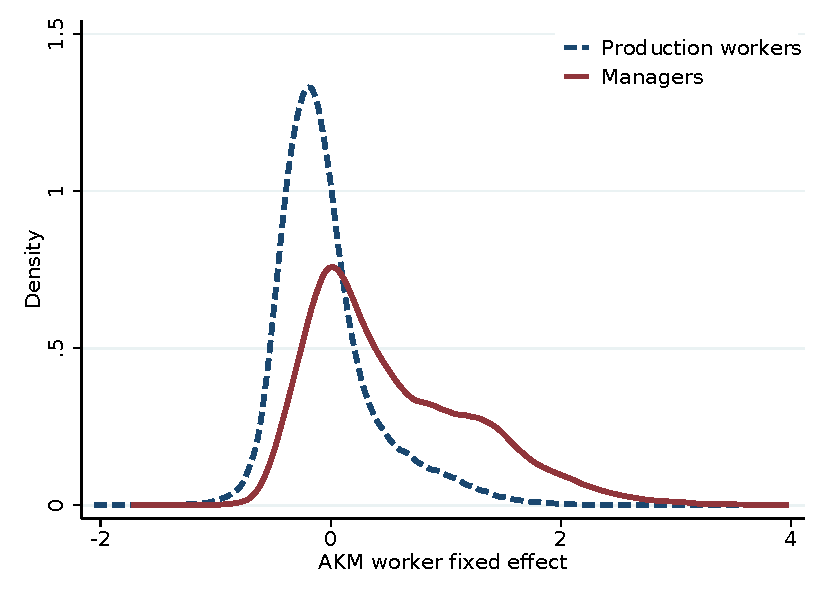
\includegraphics[width = 0.9\textwidth]{../../../figures/pe_kdensity}
    \caption{Distribution of AKM Worker Fixed Effect for Managers and Nonmanagers}
    \label{fig:pe_kdensity}
\end{figure}

\begin{figure}
    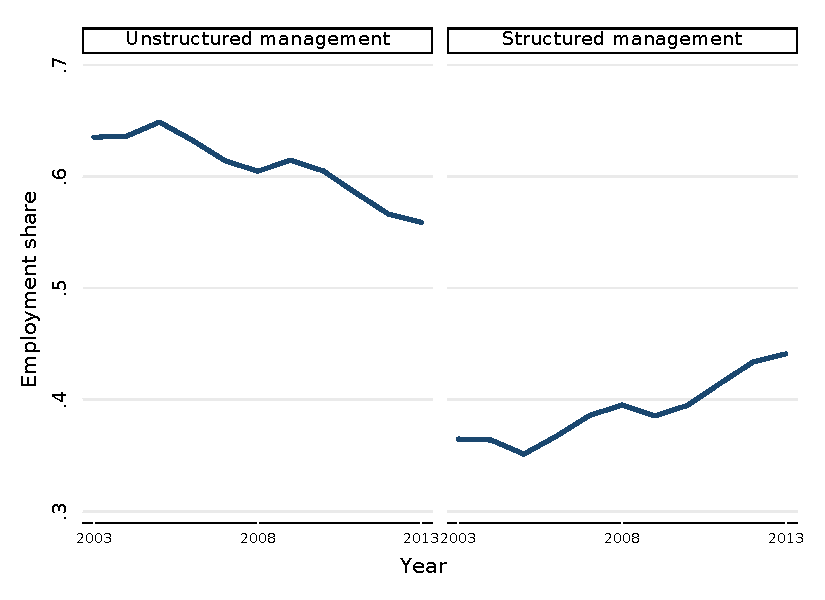
\includegraphics[width = 0.9\textwidth]{../../../figures/fig_emp_shares_struc}
    \caption{Employment shares in structured and unstructured firms}
    \label{fig:emp_shares}
\end{figure}



